\section{The fossil in the sky}\label{rep:sky}

We find that the microwave background reads the shape fossil only when the shortest cycle of the torus lies between the matched-circle bound, $0.985\,\dLSS$, and about $1.04\,\dLSS$, almost independently of the shape. %
Over the predicted distribution of shapes, the probability that the fossil is readable while matched circles stay absent peaks at $0.34$ near a present size $L_0=1.075\,\dLSS$ and exceeds $0.1$ for $1.018<L_0/\dLSS<1.183$. %
With the next-order zero-mode corrections the peak is $0.38$. %
The model does not select $L_0$, and circle and likelihood searches allow the window.
Section~\ref{rA:c-today} carries the fossil to today, Sec.~\ref{rA:c-shortest} shows that the shortest cycle decides readability, Sec.~\ref{rA:c-cov} gives the covariance and divergence, Sec.~\ref{rA:c-edges} the computed fossils and readout edges, Sec.~\ref{rA:c-ensemble} the readability over the predicted shapes, Sec.~\ref{rA:c-checks} the checks, Sec.~\ref{rA:c-size} the size of the torus, and Sec.~\ref{rA:c-tests} the tests.

\begin{figure}[tbp]
\centering
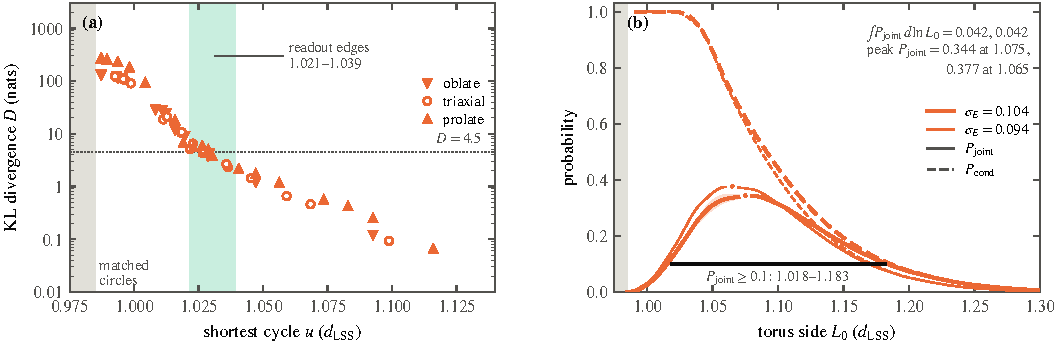
\includegraphics[width=\textwidth]{prd_fossil_sky}
\caption{Microwave-background readability of the shape fossil, set by the shortest cycle. (a)~Kullback--Leibler divergence of $55$ computed fossils from the closest circle-free cube, for temperature and $E$ modes with $2\leq\ell\leq80$ on the full sky, versus their shortest cycle $u$; band: readout edges of the 15 interpolated shapes; dotted: the readability criterion $D=4.5$; gray: excluded by matched circles. (b)~Probability that a predicted fossil is readable with no matched circles (solid) and given that circles are absent (dashed), versus the present size $L_0$, for $\sigma_E=0.104$ (thick; light band: edge-interpolation bounds) and $0.094$ (thin); bar: $P_{\rm joint}\geq0.1$. Below $L_0\simeq1.03\,\dLSS$ the dashed curve depends on the readout edge for $A<0.25$, where no fossil was computed; $P_{\rm cond}$ must vanish as $L_0\to0.985\,\dLSS$ (Sec.~\ref{rA:c-ens}).} %
\label{fig:rA-sky}
\end{figure}

\subsection{From the turning point to today}
\label{rA:c-today}

Once the Casimir force has switched off, nothing changes the shape.
Without a force the shape momenta $P_A=\MPbar^2L^3\dot\beta_A$ are conserved, so the shape velocity decays as $L^{-3}$ and the total further change of $\beta_A$, $\int P_A\,dt/\MPbar^2L^3$, converges; no homogeneous force acts on the moduli during inflation, reheating or the later expansion.
The fundamental domain today therefore has the frozen shape of Sec.~\ref{rA:s-fossil}, scaled to a present size $L_0$, which we define by its volume $L_0^3$.
Two of its properties follow from the Standard Model content and the $A_s$-calibrated plateau.
The aspect fossil is $\sigma_E=0.104$ per mode at leading order, $0.0934$ at next order and $0.059$ for free fields (Table~\ref{tab:rA-fossil}). %
The ratio $\sigma_{T_2}/\sigma_E=0.062$, or $0.11$ for free fields, keeps the edge angles sixteen (nine) times closer to $90^\circ$ than the aspect ratios are to unity. %
The size is not predicted: $L_0$ grows as $e^{N_{\rm post}}$, and $N_{\rm post}$ depends on where on the plateau the turning point sits (Sec.~\ref{rA:c-size}).

\subsection{The shortest cycle decides}
\label{rA:c-shortest}

A torus smaller than the last-scattering sphere produces pairs of matched circles~\cite{Cornish:1997ab}, and their absence requires every translation of the torus to exceed $0.985\,\dLSS$~\cite{Vaudrevange:2012da,COMPACT:2022nsu}. %
A somewhat larger torus still correlates harmonic coefficients of different $\ell$ and $m$~\cite{COMPACT:2023rkp,Himeno:2026lgh}, and these correlations carry its shape.
We computed the exact covariance of the temperature and $E$-mode coefficients for $2\leq\ell\leq80$ on the full sky, for $55$ deformed tori that cover the predicted shapes, and the Kullback--Leibler divergence $D$ of each from the circle-free cubic torus that is closest to it in this measure (Sec.~\ref{rA:c-cov}). %

\paragraph{Readability criterion.}
We call a fossil readable if $D\geq4.5$. %
For two Gaussian models of the data the expected log-likelihood ratio is $D$, so the expected $\Delta\chi^2$ is $2D$; for nested Gaussian models $2D=9$ corresponds to $3\sigma$ for a deformation of known direction, and the threshold is stricter than the $D\gtrsim3$ that Ref.~\cite{COMPACT:2022gbl} associates with a strong detection of topology. %

\paragraph{Parametrization of the fossil.}
The aspect part of the fossil lies in the $E$ plane,
\begin{equation}
\beta=A\,\sigma_E\big(\cos\theta\,X_d+\sin\theta\,X_{d2}\big),
\label{eq:rA-Eplane}
\end{equation}
with $A$ Rayleigh distributed (median $\sqrt{2\ln2}=1.177$, rms $\sqrt2$) and $\theta$ uniform for the Gaussian of Sec.~\ref{rA:s-fossil}, because the two aspect amplitudes are independent with equal widths. %
For diagonal $G=e^{2\beta}$ the sides are $L_i=L_0e^{\beta_{ii}}$, and Eq.~\eqref{eq:rA-XE} gives
\begin{equation}
\beta_{ii}=\sqrt{\tfrac23}\,A\sigma_E\cos(\theta-\theta_i),\qquad \theta_i=30^\circ,\ 150^\circ,\ 270^\circ,
\end{equation}
so the sides are $L_0\exp[\sqrt{2/3}\,A\sigma_E\cos(\theta-\theta_i)]$, and we write $u$ for the shortest of them.
The cubic group acts on this plane as the dihedral group of order six, generated by rotations by $120^\circ$, which permute the edges, and by reflections.
Its invariants are $\Tr\beta^2=A^2\sigma_E^2$ and $\Tr\beta^3=(2/3)^{3/2}\sum_i\cos^3(\theta-\theta_i)A^3\sigma_E^3=\tfrac34(2/3)^{3/2}A^3\sigma_E^3\sin3\theta$, so every observable depends on $\beta$ through $A^2$ and $A^3\sin3\theta$, and $-\pi/6\leq\theta\leq\pi/6$ covers all shapes.
At $\theta=\pi/6$ one side is long and two are short (prolate), at $\theta=-\pi/6$ two are long and one is short (oblate), and $\theta=0$ is triaxial.
The angle modes change $D$ only at second order, by about $0.4\%$ for $\sigma_{T_2}=0.0065$, and we neglect them (Sec.~\ref{rA:c-edges}). %

\paragraph{Result.}
We find that the divergence is a steep function of $u$ and depends on the amplitude and orientation of the fossil almost only through it [Fig.~\ref{fig:rA-sky}(a)].
Near the circle bound, $u\simeq0.99\,\dLSS$, it is $D\simeq90$--$270$ for every computed amplitude from $A=0.25$ to $2$; it falls to about $4.5$ at $u\simeq1.027\,\dLSS$, to $1$ at $1.05$ and to $0.1$ at $1.10\,\dLSS$. %
Over the $15$ computed shapes the readout edge $u_{\max}$, the shortest cycle at which $D=4.5$, lies between $1.021$ and $1.039\,\dLSS$, and between $1.023$ and $1.032\,\dLSS$ for $A\geq0.5$ (Table~\ref{tab:rA-edges}). %
A fit to all points with $0.2<D<80$ gives
\begin{equation}
\ln D=3.25+0.07\ln A-56\,(u/\dLSS-1)-0.05\sin3\theta
\end{equation}
with a scatter of $0.34$. %
What the maps resolve is set by how close the nearest image comes; the amplitude and orientation of the fossil decide mainly at which $L_0$ that happens.
Near the edge $\ln D$ falls by $85$--$130$ per unit of $u/\dLSS$, so doubling the information moves the edge outward by only about $0.008\,\dLSS$. %

\subsection{Covariance and divergence}
\label{rA:c-cov}

\paragraph{Covariance on the torus.}
For a torus with lattice basis $B=L_0G^{1/2}$ the allowed wave vectors are $\bm k_{\bm n}=2\pi B^{-\mathsf T}\bm n$.
The primordial curvature perturbation is a Fourier series, and the harmonic coefficients of the temperature and $E$ modes, $X\in\{T,E\}$, follow from it with the transfer functions $\Delta^X_\ell$:
\begin{equation}
\zeta(\bm x)=\sum_{\bm n}\zeta_{\bm n}e^{i\bm k_{\bm n}\cdot\bm x},\qquad \langle\zeta_{\bm n}\zeta^*_{\bm n'}\rangle=\frac{P_\zeta(k_{\bm n})}{L_0^3}\,\delta_{\bm n\bm n'},\qquad
a^X_{\ell m}=4\pi i^\ell\sum_{\bm n}\Delta^X_\ell(k_{\bm n})\,\zeta_{\bm n}\,Y^*_{\ell m}(\hat{\bm k}_{\bm n}).
\end{equation}
Their covariance is therefore~\cite{COMPACT:2023rkp}
\begin{equation}
C^{XY}_{\ell m,\ell'm'}=\frac{(4\pi)^2}{L_0^3}\,i^{\ell-\ell'}\sum_{\bm n\neq0}P_\zeta(k_{\bm n})\,\Delta^X_\ell(k_{\bm n})\Delta^Y_{\ell'}(k_{\bm n})\,Y_{\ell m}(\hat{\bm k}_{\bm n})\,Y_{\ell'm'}(\hat{\bm k}_{\bm n})
\label{eq:rA-cov}
\end{equation}
in a real harmonic basis; the zero mode $\bm n=0$ carries no fluctuation.
The transfer functions $\Delta^X_\ell$ of unlensed scalar perturbations are computed with CAMB~\cite{Lewis:1999bs} for the Planck 2018 $\Lambda$CDM parameters~\cite{Planck:2018vyg}.
CAMB sets $\Delta_\ell$ to zero below $k\chi_*\simeq14$ for $18\leq\ell\leq26$, and we continue it there with the spherical Bessel asymptotics, which matters for the few lowest torus modes. %
Modes with $k\chi_*>x_{\max}$ are replaced by the isotropic continuum through a smooth taper over the last quarter of that range, which makes $C$ a smooth function of the shape; for $\ell\leq80$ we use $x_{\max}=240$. %
At $L_0=6\,\dLSS$ the construction reproduces the covering-space spectra with $D\sim10^{-6}$. %

\paragraph{Block structure.}
For a diagonal $G$, which includes every shape of Eq.~\eqref{eq:rA-Eplane}, each coordinate reflection maps the lattice to itself and leaves $P_\zeta$, $\Delta_\ell$ and the taper invariant.
Under $x\to-x$ the azimuth goes to $\pi-\varphi$, so $\cos m\varphi$ picks up $(-1)^m$ and $\sin m\varphi$ picks up $(-1)^{m+1}$; under $y\to-y$, $\varphi\to-\varphi$ flips only the sine harmonics; and under $z\to-z$, $P^m_\ell$ picks up $(-1)^{\ell+m}$.
Real harmonics therefore carry the character $(|m|+[m<0],\,[m<0],\,\ell+|m|)$ mod $2$ under the three reflections, and sums over orbits of different characters vanish.
The covariance therefore splits exactly into eight blocks, and the divergence is the sum of the block divergences.
At a generic point of the $E$ plane, $(A,\theta)=(1.3,0.37)$, the whitened elements between different characters are below $1.6\times10^{-16}$, and the full-matrix divergence equals the sum over blocks to all printed digits. %

\paragraph{Divergence.}
The divergence of a fossil covariance $C_\beta$ from a reference $C_0$ is
\begin{equation}
D(C_\beta\|C_0)=\tfrac12\Big[\Tr\big(C_0^{-1}C_\beta\big)-n-\ln\det\big(C_0^{-1}C_\beta\big)\Big],
\label{eq:rA-kl}
\end{equation}
with $n$ the dimension, the expected log-likelihood ratio of the two zero-mean Gaussian models when the data follow $C_\beta$.
We evaluate it from traces and log-determinants of packed inverses to a relative accuracy of $1.7\times10^{-12}$. %
The fixed divergence uses the cube of equal volume.
The profiled divergence minimizes over the side $s'\geq0.985\,\dLSS$ of a circle-free cube aligned with the axes of the fossil, over a pool of $19$ cubes spaced by at most $0.015\,\dLSS$. %
A bracketed Brent search on three fossils at the edge finds interior minima $0.04$--$0.55\%$ below the pool minima, which moves the edges by at most $6\times10^{-5}\,\dLSS$. %
A three-point parabolic refinement undershoots where the profile rises steeply toward the circle bound, so we use the pool minima.
Profiling lowers the integrated measure, Eq.~\eqref{eq:rA-measure}, from $0.0442$ to $0.0422$, and a free overall amplitude of the spectrum is optimal at $1.0000$--$1.0006$ and changes nothing. %

\paragraph{Fisher matrix.}
At the cube the Fisher matrix
\begin{equation}
F_{AB}=\tfrac12\Tr\big(C^{-1}\partial_AC\,C^{-1}\partial_BC\big)
\label{eq:rA-fisher}
\end{equation}
is block diagonal in the $E$, $T_2$ and rotation ($T_1$) representations of the cubic group.
For $\ell\leq30$ the uncertainty of one aspect amplitude is $\sigma(\beta_E)=0.023$, $0.073$ and $0.25$ at $L_0=1.05$, $1.1$ and $1.2\,\dLSS$, and the angle fossil, $0.0065$ per mode, stays below its $1\sigma$ uncertainty at every size allowed for a typical fossil. %
Near the circle bound the quadratic Fisher estimate misjudges deformations of fossil size by factors between $0.2$ and $3$, which is why we use the exact divergence. %

\subsection{Fossils and readout edges}
\label{rA:c-edges}

We computed $55$ fossils with $A\in\{0.25,0.5,1,\sqrt2,2\}$ and $\theta\in\{-\pi/6,0,\pi/6\}$, each at two to six sizes with $u\simeq0.987$--$1.12\,\dLSS$, including slices at $L_0=1.13$, $1.14$ and $1.15\,\dLSS$, against the $19$ reference cubes. %
Table~\ref{tab:rA-edges} lists the readout edges.
For $A=0.25$ both computed sizes lie above the threshold, and the edge is extrapolated upward, with the last chord as lower bound and a shallow slope of $60$ per unit of $u/\dLSS$ as upper bound. %
For the other amplitudes the chord between the computed sizes bounds the edge from above and the extension of the steeper preceding segment from below.

\begin{table}[tbp]
\centering
\caption{Readout edge $u_{\max}/\dLSS$, the shortest cycle at which $D=4.5$, for temperature and $E$ modes with $\ell\leq80$ and the profiled reference cube, at amplitude $A$ of Eq.~\eqref{eq:rA-Eplane}. Ranges are convex bounds from the computed sizes; the row $A=0.25$ is extrapolated.}
\label{tab:rA-edges}
\begin{tabular}{lccc}
\toprule
$A$ & oblate & triaxial & prolate\\
\midrule
$0.25$ & $1.0282$--$1.0393$ & $1.0233$--$1.0350$ & $1.0214$--$1.0259$\\ %
$0.5$ & $1.0275$--$1.0322$ & $1.0229$--$1.0242$ & $1.0247$--$1.0275$\\ %
$1$ & $1.0271$ & $1.0262$ & $1.0287$\\ %
$\sqrt2$ & $1.0253$--$1.0279$ & $1.0263$--$1.0272$ & $1.0287$--$1.0302$\\ %
$2$ & $1.0289$ & $1.0279$--$1.0282$ & $1.0300$--$1.0308$\\ %
\bottomrule
\end{tabular}
\end{table}

\paragraph{No polynomial law in the window.}
At fixed $L_0$ the leading invariants allowed by the cubic symmetry far from the circle bound motivate a fit $D=c_2A^2+c_3A^3\sin3\theta+c_4A^4$.
In the window this fit fails: at $L_0=1.14\,\dLSS$ its relative residuals have an rms of $4.9$, and it predicts negative $D$ for prolate shapes. %
There the orientations differ by their shortest cycles, so the divergence of a single fossil and its dependence on $\ell_{\max}$ cannot be carried over to the ensemble by a polynomial in $A$.

\paragraph{Angle modes.}
On diagonal shapes each angle direction $X_{ij}$ is odd under two reflections and couples different characters, so the angle modes change $D$ only at second order.
For the typical fossil at $L_0=1.13\,\dLSS$ and $\ell\leq40$, an angle amplitude $0.0065$ along $X_{12}$ lowers $D$ by $0.12\%$, and twice that amplitude by $0.50\%$, a ratio of $3.996$, as expected for a quadratic effect. %
With the ratio $F_{T_2}/F_E=0.647$ at the cube, the expected angle contribution is about $0.4\%$ of the aspect one. %

\subsection{Readability over the predicted shapes}
\label{rA:c-ensemble}

At a given present size the fossil is readable if $0.985\,\dLSS\leq u\leq u_{\max}$. %
Averaging over the Gaussian distribution of Eq.~\eqref{eq:rA-Eplane} gives the joint probability $P_{\rm joint}(L_0)$ that the fossil is readable and matched circles are absent, and the conditional probability $P_{\rm cond}$ given that circles are absent [Fig.~\ref{fig:rA-sky}(b)].
For temperature and $E$ modes to $\ell=80$, $P_{\rm joint}$ peaks at $0.344$ near $L_0=1.075\,\dLSS$, with bounds $0.339$--$0.351$ from the interpolation of the readout edges, and it never reaches one half. %
It exceeds $0.3$ for $1.048<L_0/\dLSS<1.105$, $0.2$ for $1.033$--$1.140$ and $0.1$ for $1.018$--$1.183$. %
Given that circles are absent, the fossil is readable with probability above one half up to $L_0=1.090\,\dLSS$, and with probability $0.44$, $0.32$, $0.23$ and $0.16$ at $L_0=1.10$, $1.12$, $1.14$ and $1.16\,\dLSS$. %
Below about $1.03\,\dLSS$ the conditional probability rests on an extrapolation of the readout edge to amplitudes $A<0.25$, but there at most a fifth of the fossils are free of circles (Sec.~\ref{rA:c-ens}). %

\paragraph{The integrated measure.}
Averaging over shapes spreads the readable sizes without adding to them.
For a fixed shape $\ln u=\ln L_0+\min_i\beta_{ii}$, so the readable range of $\ln L_0$ is an interval of width $\ln(u_{\max}/0.985\,\dLSS)$, shifted by the shape; integrating $P_{\rm joint}$ over $\ln L_0$ and then averaging over shapes gives
\begin{equation}
\int P_{\rm joint}\,d\ln L_0=\Big\langle\ln\frac{u_{\max}}{0.985\,\dLSS}\Big\rangle=0.042,
\label{eq:rA-measure}
\end{equation} %
almost exactly the width, $0.0415$, of the window of a single typical fossil, $|\beta_E|=\sqrt2\,\sigma_E$ along $X_d$, which is readable for $1.093<L_0/\dLSS<1.139$. %
The distribution of shapes turns that window into a band with a peak probability of about one third, $3.6$ times wider in $\ln L_0$ at the $0.1$ level. %
Inside the window of the typical fossil the joint probability falls from about one third to one fifth, because there smaller fossils have their shortest cycle beyond the edge and larger ones have circles. %
At the peak, $L_0=1.075\,\dLSS$, the typical fossil itself has circles; the readable fossils there have $u$ between $0.985$ and about $1.027\,\dLSS$, with $A\simeq0.5$--$1.2$ for oblate and triaxial and $A\simeq1.0$--$2.1$ for prolate shapes. %

\paragraph{Next order.}
The next-order zero-mode corrections shrink the fossil to $\sigma_E=0.0934$ (Sec.~\ref{rA:s-fossil}). %
With $\sigma_E=0.094$ the peak rises to $0.377$ near $L_0=1.065\,\dLSS$ and the $0.1$ level spans $1.015$--$1.168\,\dLSS$. %
The integrated measure, $0.0421$, does not change, since Eq.~\eqref{eq:rA-measure} depends only on the readout edges. %
A $10\%$ smaller (larger) $\sigma_E$ raises (lowers) the peak by about $9$--$10\%$ and moves the upper end of the $0.1$ range by $-0.013$ ($+0.015$)\,$\dLSS$. %

\paragraph{Information used.}
The conclusion depends little on the information used.
From $\ell\leq30$ to $\ell\leq80$ the divergence of the typical fossil at $L_0=1.13\,\dLSS$ grows by a factor of about $2.2$. %
The peak probability, the integrated measure and the conditional probability at $1.10\,\dLSS$ grow only by factors $1.23$--$1.31$, because more information moves the readout edge only slightly. %
White noise and beams of the Planck $143$\,GHz type lower the peak to $0.313$ and the integrated measure by $9\%$; temperature alone gives $0.286$ and $0.035$ (Table~\ref{tab:rA-variants}). %
Masks, foregrounds and the uncertainty of the reionization optical depth, which dominates the lowest $E$ multipoles, are not included; they reduce the information and lower these probabilities further.

\begin{table}[tbp]
\centering
\caption{Readability over the predicted shapes: peak of $P_{\rm joint}$ with its position $L_0/\dLSS$, the range of $L_0/\dLSS$ with $P_{\rm joint}\geq0.1$, and the integrated measure, Eq.~\eqref{eq:rA-measure}. TE80 denotes temperature and $E$ modes with $\ell\leq80$, and so on; the reference cube is profiled except in the second row (equal volume). Noise is white with a Gaussian beam of the Planck $143$\,GHz type. All rows use $\sigma_E=0.1041$ except the last.}
\label{tab:rA-variants}
\begin{tabular}{lccc}
\toprule
Readout & $P_{\rm joint}^{\max}$ & $P_{\rm joint}\geq0.1$ & Measure\\
\midrule
TE80 & $0.344$ ($1.075$) & $1.018$--$1.183$ & $0.0422$\\ %
TE80, fixed & $0.360$ ($1.078$) & $1.018$--$1.185$ & $0.0442$\\ %
TE40 & $0.305$ ($1.075$) & $1.018$--$1.178$ & $0.0377$\\ %
TE30 & $0.264$ ($1.078$) & $1.020$--$1.168$ & $0.0325$\\ %
T80 & $0.286$ ($1.078$) & $1.018$--$1.173$ & $0.0352$\\ %
TE80, noise & $0.313$ ($1.075$) & $1.018$--$1.178$ & $0.0384$\\ %
TE30, noise & $0.190$ ($1.080$) & $1.035$--$1.150$ & $0.0228$\\ %
TE80, $\sigma_E=0.094$ & $0.377$ ($1.065$) & $1.015$--$1.168$ & $0.0421$\\ %
\bottomrule
\end{tabular}
\end{table}

\subsubsection{Ensemble method}
\label{rA:c-ens}

The ensemble uses $2\times10^6$ shapes drawn from Eq.~\eqref{eq:rA-Eplane} with $\sigma_E=0.1041$, which gives a binomial error below $3.4\times10^{-4}$. %
Within each $\theta$ the readout edge is interpolated piecewise linearly in $A$, extrapolated linearly below $A=0.25$ and held constant above $A=2$, and it is interpolated quadratically in $\sin3\theta$ through the three computed orientations; the grid in $L_0$ has steps of $0.0025\,\dLSS$. %
The convex bounds on the edges give the bounds $0.339$--$0.351$ on the peak of $P_{\rm joint}$. %
This ensemble is the predicted distribution, in which the two aspect amplitudes of a rectangular torus are independent with equal widths and the angle amplitudes are sixteen times narrower.
It differs from the eigenvalue law of an isotropic five-component deformation, which carries a Vandermonde factor $\propto A^3|\cos3\theta|$ and gives non-rectangular lattices. %
Table~\ref{tab:rA-variants} summarizes the readouts.

For $L_0\leq1.03\,\dLSS$ the conditional probability depends on the readout edge for $A<0.25$, where no fossil was computed.
At $L_0=1.00$ and $1.02\,\dLSS$ it is $0.956$ and $0.945$ for $D\propto A^2$, $1.00$ and $0.997$ for the linear extrapolation used in the ensemble, and $0.12$ and $0.76$ in the extreme case that such fossils are unreadable. %
It must vanish as $L_0\to0.985\,\dLSS$, where only fossils close to the cube, with $D\to0$, are free of circles.
The lower end of the range $P_{\rm cond}\geq1/2$ thus lies between $0.986$ and $1.009\,\dLSS$, while the upper ends, $1.090$, $1.1225$, $1.1475$ and $1.185\,\dLSS$ for $P_{\rm cond}\geq0.5$, $0.3$, $0.2$ and $0.1$, are robust. %
The joint probability is affected only below $L_0\simeq1.03\,\dLSS$, where it is at most $0.2$. %

\subsection{Checks}
\label{rA:c-checks}

Our covariance code reproduces the stored covariance matrices of an earlier single-fossil analysis (Sec.~\ref{rep:v-conditional}).
For the typical fossil at $L_0=1.13\,\dLSS$ and $x_{\max}=320$ it gives $D=11.3495$ for $\ell\leq80$, equal to the cached value to $2\times10^{-14}$, and a fresh build agrees with the cached matrix to $2\times10^{-16}$ after whitening. %
At the edge of the typical fossil, $L_0=1.14\,\dLSS$, raising $x_{\max}$ from $240$ to $320$ changes the profiled divergence for $\ell\leq80$ by $-0.69\%$, and halving the taper changes it by $+0.17\%$. %
This moves the edge by about $10^{-4}\,\dLSS$; the other edges lie in the same regime near the circle bound, but only this one was tested. %
An independent build with CAMB~2.0.5 reproduces the divergence of the typical fossil at $L_0=1.13\,\dLSS$ for $\ell\leq40$, $7.226$, to $0.10\%$. %
An independent implementation of the ensemble from the tabulated divergences gives a peak of $0.350$ near $L_0=1.076\,\dLSS$, $P_{\rm joint}\geq0.1$ for $1.016$--$1.184\,\dLSS$ and an integrated measure of $0.0421$. %
For $\ell\leq30$ a separate temperature-only code, with a sharp cutoff and its own transfer functions, harmonics and mode sums, reproduces the Fisher widths at the cube to $1\%$ at $L_0=1.1\,\dLSS$ and $7\%$ at $1.2\,\dLSS$, and the divergence between the cubic torus and the covering space to $1\%$ for $1\leq L_0/\dLSS\leq1.3$. %
The noise of Table~\ref{tab:rA-variants} is white, $33$ and $70\,\mu$K\,arcmin for temperature and polarization, with an isotropic Gaussian beam of $7.3'$ full width at half maximum, which preserves the block structure; masks would break it and are not included. %
Further convergence data are collected in Sec.~\ref{rep:v-convergence}.

\subsection{The size of the torus}
\label{rA:c-size}

The model fixes the width of the distribution of present sizes but not its center.

\paragraph{A family of turning points.}
Time symmetry about the turn, $\Theta$ of Sec.~\ref{rA:s-equivalent}, sets $\dot\phi=\dot\beta=0$ there in a classical history.
The constraint at the turn, $V(\phi_b)\Lb^4=\rANeff\rAgam$, then leaves a one-parameter family of turning points labeled by the inflaton value $\phi_b$.
As $\phi_b$ runs from $4.9$ to $6.3\,\MPbar$, the number of $e$-folds after the turn grows from $38$ to $125$ while $\Lb$ changes by $0.6\%$, and $A_s$ fixes $h$ at the pivot independently of $\phi_b$. %
The center $\phi_b$ therefore sets $N_{\rm post}-N_*$, that is $\ln L_0$.
Neither the constraint, nor time symmetry and the reality conditions of Sec.~\ref{rA:s-equivalent}, nor $A_s$ selects $\phi_b$, and the minimal-energy-variance rule, applied to the center, has no interior minimum and drives $\phi_b$ to infinity.
Since $dN_{\rm post}/d\phi_b=58/\MPbar$ there, landing in the window of the typical fossil, $0.0415$ $e$-fold wide, requires $\phi_b$ to within $0.0415/58=7\times10^{-4}\,\MPbar$. %

\paragraph{A lower bound on the width.}
The width, in contrast, has a lower bound.
To linear order $N_{\rm post}-\bar N=\mathcal A\,\delta\phi_b+\mathcal B\,\delta P_b$, where $P_b$ is the momentum of the inflaton zero mode at the turn and $[\phi_b,P_b]=i$.
Time reversal maps $Q=\mathcal A\phi_b+\mathcal BP_b$ to $\bar Q=\mathcal A\phi_b-\mathcal BP_b$, so in a $\Theta$-invariant state, pure or mixed, $Q$ and $\bar Q$ have the same distribution, while
\begin{equation}
[Q,\bar Q]=-\mathcal A\mathcal B[\phi_b,P_b]+\mathcal B\mathcal A[P_b,\phi_b]=-2i\mathcal A\mathcal B .
\end{equation}
The uncertainty relation $\rAVar\,Q\,\rAVar\,\bar Q\geq\tfrac14|\langle[Q,\bar Q]\rangle|^2$ with $\rAVar\,Q=\rAVar\,\bar Q$ then gives
\begin{equation}
\sigma_N^2\geq|\mathcal A\mathcal B|,
\label{eq:rA-sizebound}
\end{equation}
provided the other sectors are uncorrelated with $(\phi_b,P_b)$ at linear order; the bound does not require a Gaussian state.
At the reference turning point it gives $\sigma_N\geq0.935$ $e$-fold, $0.938$ in the window of the typical fossil, and about $0.0137\,N_{\rm post}$ in general. %
The time-symmetric Gaussian of minimal energy variance (Sec.~\ref{rA:s-equivalent}), applied to the inflaton zero mode, whose energy spread is dominated by the slope of the plateau, gives $\sigma_N=0.959$, $2.5\%$ above the bound. %

\paragraph{Measures on the center.}
Probabilities need a measure on $\phi_b$.
For an amplitude independent of $\phi_b$, the Liouville measure on the turning surface, the Klein--Gordon norm of the expanding branch, the Schr\"odinger norm on a slice of fixed volume and the inverse-potential norm of Ref.~\cite{Godet:2026gqw} all give $p(N_{\rm post})\simeq1.17/N_{\rm post}$ for $38\leq N_{\rm post}\leq125$, which cannot be normalized on the plateau. %
With a cutoff the probability of a readable fossil, given that circles are absent, falls from $1.4\times10^{-3}$ for $N_{\rm post}\leq100$ to $5\times10^{-5}$ for $N_{\rm post}\leq10^6$. %
The only dependence on $\phi_b$ in the equations of the torus itself is the WKB factor $e^{\pm2S_E}$ of the Casimir-forbidden region $L<\Lb$, with $S_E\simeq1.2\times10^4$, and its sign is set by the inner boundary data, not by time symmetry. %
The growing sign, which resembles the no-boundary weight, gives $6.1\%$, and the decaying sign at most $6\times10^{-19}$. %
A time-symmetric Gaussian state of minimal width gives at most $1.5\%$ wherever it is centered. %
These rates use the readout edges for $\ell\leq30$; the edges for $\ell\leq80$ raise them by about a factor $1.2$. %

\paragraph{Priors on the size.}
For any prior on $\ln L_0$ that is broad on the scale of the window, the probability $P_{\rm cond}$ of a readable fossil given that circles are absent is the prior density, normalized to the sizes without circles, times the integrated measure, Eq.~\eqref{eq:rA-measure}.
A Gaussian of width $0.95$ in $\ln L_0$ centered at $1.13\,\dLSS$, about the width $\sigma_N=0.959$ of the model's own state of minimal energy variance above, gives $P_{\rm cond}\approx3.3\%$. %
The width $1.909$ of the inflaton packet of Sec.~\ref{rep:v-conditional}, which is what the same rule gives when the slope of the plateau is neglected, yields about $1.7\%$, and a prior $\propto L_0^{-\alpha}$ reaches $P_{\rm cond}=1/2$ only for $\alpha\simeq17.6$. %
An exponential prior of the no-boundary type with slope $3.2\times10^{-4}$ gives $1.3\times10^{-5}$, and the flat measure above with $N_{\rm post}\leq10^3$ gives $2.3\times10^{-4}$. %
These priors are conditional experiments, not measures derived from a wave function.
The values above use the parabolic profiles; the pool minima raise them by $2.3\%$. %
Relative to the readout edges for $\ell\leq30$, which the rates of the previous paragraph use, the edges for $\ell\leq80$ raise the probability of a readable fossil under broad priors by about a factor $1.2$, for instance from $1.4\%$ to $1.7\%$ for the Gaussian of width $1.909$. %
A readable fossil therefore needs a prior on the size sharply concentrated near the circle bound, and the model provides none.

\subsection{Present searches and tests}
\label{rA:c-tests}

Present searches allow the window.
For a cubic torus the Planck 2013 likelihood requires $L>0.92\,\dLSS$~\cite{Planck:2013okc}, the Planck 2015 likelihood $L>0.97\,\dLSS$~\cite{Planck:2015gmu}, and the absence of matched circles $L>0.985\,\dLSS$~\cite{COMPACT:2022nsu}. %
A shortest cycle between $0.985$ and about $1.04\,\dLSS$ is therefore allowed by circle and likelihood searches, and it lies within the range $L\lesssim1.2\,\dLSS$ where off-diagonal correlations remain detectable in principle~\cite{COMPACT:2023rkp}; no published analysis has excluded it. %

If a torus is found with its shortest cycle in this window, its fundamental domain should be close to a rectangular box.
Its aspect amplitudes should be compatible with an isotropic Gaussian of width $0.104$ per mode ($0.094$ at next order), truncated at large elongation by the absence of circles, and its angles should lie within about a degree of $90^\circ$. %
Angle deviations above about $20^\circ$, which the multipoles $\ell\leq30$ alone detect at $3\sigma$ for $L_0=1.10\,\dLSS$, would exclude the natural state. %
A single sky is one draw from the predicted distribution.
For two independent Gaussian amplitudes of width $\sigma_E$ the score of $\ln\sigma_E$ is $\sum_i(\beta_i^2/\sigma_E^2-1)$, whose variance is $2$ per amplitude, so the Fisher information on $\ln\sigma_E$ from the two aspect amplitudes of one torus is $4$, and even a perfect measurement tests the predicted width only to about $50\%$. %
A null topology search out to a shortest cycle of about $1.05\,\dLSS$ would close the window.
The Casimir sector leaves no other trace: its contribution to $\Delta N_{\rm eff}$ is negligible, and the primordial spectra are those of the plateau (Sec.~\ref{rep:spectra}).
